\chapter{Arquitetura do Ambiente de DWing}
\label{arquitetura}


Para a implementação do ambiente do DWing para métricas de código-fonte, foi definida a arquitetura tal como se mostra Figura \ref{arquitetura}.


\begin{figure}[ht!]
\centering
\includegraphics[keepaspectratio=false,scale=0.20]{figuras/arquitetura-dwing.eps}
\caption{Arquitetura do Ambiente de DWing para Métricas de Código-Fonte}
\label{arquitetura}
\end{figure}
\FloatBarrier

Para selecionar as ferramentas, que implementarão cada um dos componentes do ambiente DWing, estabeleceram-se critérios gerais de seleção tal como pode ser visto na Tabela \ref{seleção}.


	\begin{table}[!ht]
	\begin{center}
	 \begin{tabular}{|l|l|}
		\hline
		Identificador & Critério 
		\\ \hline
		CG01 & A ferramenta deve possuir código aberto.  
		\\ \hline
		CG02 & A ferramenta deve ter documentação disponível em inglês ou português.      
		\\ \hline
		CG03 & A ferramenta deve possuir uma comunidade ativa em seu uso.
		\\ \hline
		CG04 & A ferramenta deve possuir releases estáveis.    
		\\ \hline
		\end{tabular}
		\caption{Critérios Gerais de seleção de ferramentas}
		\label{seleção}
		\end{center}
		\end{table}	


\section{Ferramenta de Análise Estática de Código-Fonte}

Além dos critérios gerais estabelecidos para escolha da ferramenta de análise estática de código-fonte, que é a fonte externa de coleta dos dados, estabeleceram-se os critérios específicos para seleção de ferramentas de análise estática de código fonte (CAE) apresentados na Tabela \ref{specific}.


	\begin{table}[!ht]
	\begin{center}
	 \begin{tabular}{|l|p{10cm}|}
		\hline
		Identificador & Critério 
		\\ \hline
		CAE01 & A ferramenta deve prover as métricas de código-fonte para as linguagens de programação, tal como especificado na Tabela \ref{metrics}.
		\\ \hline
		CAE02 & A ferramenta deve possuir saída de dados em arquivo em alguns dos seguintes formatos: JSON, XML, TXT, CSV.      
		\\ \hline
		\end{tabular}
		\caption{Critérios Específicos para Ferramenta de Análise Estática de Código-Fonte}
		\label{specific}
		\end{center}
		\end{table}	

Após a realização de uma busca por ferramentas de análise estática de código-fonte, foram pre-selecionados o SonarQube~\footnote{Disponível em \url{http://www.sonarqube.org/}} e Analizo~\footnote{Disponível em \url{http:/http://analizo.org/}} cujas principais características de ambas são apresentadas na Tabela \ref{dados-ferramentas-estatica}.

\begin{savenotes}
\begin{table}[!ht]
\centering
\begin{tabular}{|p{5cm}|p{4.5cm}|p{5cm}|}
\hline

Característica 

&

\begin{center}

\includegraphics[keepaspectratio=true,scale=0.48]{figuras/analizo.eps} 
\end{center}


&



\begin{center}

\includegraphics[keepaspectratio=true,scale=0.48]{figuras/sonarqube.eps} 
\end{center}





   
\\ \hline


%--------------------------
Linguagens com Suporte  & C, C++, Java & C, C++, Java, PHP,Scala, Python, Delphi, Pascal, Flex, ActionScript, Javascript, Groovy~\footnote{O SonarQube oferece suporte comercial a outras linguagens, contudo foram listadas apenas que tem suporte por meio de \textit{plugins} de código-aberto} \\ \hline
Licença  & GNU GPL3 & GNU LGPL3  \\ \hline



%-----------------------------------

Métricas de Código-Fonte fornecidas  & 25 métricas em âmbito de Projeto e 16  métricas em âmbito de Classe \cite{Meirelles2013} & 12 métricas em âmbito de Classe, 8 métricas em âmbito de projeto \footnote{O SonarQube forneceu suporte as estas métricas até a versão 4}. \\ \hline


%--------------------------
Formato de Saída das Métricas  & YAML, CSV & JSON, XML \\ \hline

%--------------------------
Plataforma  &   GNU Linux (homologado para distribuições baseadas em Debian). & Windows, Linux, Mac OS X e Servidores de Aplicação Java                                                                                              \\ \hline

%--------------------------
Integração com outras ferramentas & Mezuro, Kalibro & Jenkins, Hudson, Mantis, JIRA, Crowd e entre outros \\ \hline

%--------------------------

%--------------------------
Sistema de Controle de Versões & Git & Git \\ \hline

%--------------------------
Idioma com Suporte & Inglês & Inglês, Português, Japonês, Italiano, Chinês, Francês, Grego e Espanhol \\ \hline

%------------------------
Idioma da Documentação & Inglês & Inglês

\\ \hline
%-----------------------
Última Versão Estável em 10/05/2013 & 1.18.0 & 4.2

\\ \hline
\end{tabular}
\caption{Características do SonarQube e do Analizo}
\label{dados-ferramentas-estatica}
\end{table}
\FloatBarrier
\end{savenotes}

Tendo as características gerais de cada ferramenta levantadas, foram comparadas (SonarQube e Analizo) quanto aos critérios gerais e aos critérios específicos para ferramentas de análise estática, tal como se mostra na Tabela \ref{compare}.


\begin{table}[!ht]
\centering
\begin{tabular}{|l|l|l|}
\hline
Critérios & SonarQube  & Analizo    \\ \hline
CG01      & \checkmark & \checkmark \\ \hline
CG02      & \checkmark & \checkmark \\ \hline
CG03      & \checkmark & \checkmark \\ \hline
CG04      & \checkmark & \checkmark \\ \hline
CAE01     & \checkmark & \checkmark \\ \hline
CAE02     & \checkmark & \checkmark \\ \hline
\end{tabular}
\caption{Análise do SonarQube e do Analizo quanto aos critérios gerais e quanto aos critérios específicos de ferramentas de análise estática}
\label{compare}
\end{table}
\FloatBarrier

\todo[inline, color=yellow!50]{Descrever o porquê da Escolha do Analizo}


\section{Projeto do \textit{Data Warehouse}}

O \textit{Data Warehouse} como elemento central do ambiente de \textit{Data Warehousing} deve ser o primeiro a ser projetado \cite{Kimball2002}. Isso ocorre pois o DW deve ser dirigido ao negócio. Logo a modificação do DW impacta principalmente na carga dos dados, na etapa de extração, transformação e carga, requerendo modificações conforme o DW venha a mudar.

Seguindo a metolodogia proposta por \citeonline{Kimball2002}, apresentada na seção \ref{metodologia-dw}, entende-se que o processo de negócio a ser avaliado é o monitoramento da qualidade do código-fonte expresso por meio das métricas de código-fonte. 


\todo[inline, color=yellow!50]{Atualizar a seção com as informações de hierarquia, entidades de negócio, granularidade, dimesões e fatos}



\section{Ferramentas de DWing}

Tendo em vista que o \textit{Data Warehouse} foi projetado em um modelo dimensional, é possível construir tanto o processo de \textit{Extraction-Transformation-Load} quanto as operações de consulta OLAP. Entre as alternativas de código aberto que suportam este ambiente como um todo, está o Pentaho BI Suite Community Edition. Este apresenta soluções que cobrem 
as áreas de ETL, \textit{reporting}, OLAP e mineração de dados. Cada um dos componentes utilizados é apresentado e analisado nas seções subsequentes.
 


\subsection{Implementação da Extração, Transformação e Carga dos Dados}
\label{implementação-ETL}
O Pentaho Data Integration Community Edition ou Kettle\footnote{Disponível em \url{http://kettle.pentaho.com/}}, como é conhecido pela comunidade que o desenvolve, é feito na linguagem Java e implementa o processo de ETL (Extração, Transformação e Carga de Dados). A interface do Kettle é mostrada na Figura \ref{pdi} e as principais características do Kettle e a análise quanto aos critérios gerais de seleção de ferramentas são apresentadas na Tabela \ref{kettle}.

\begin{figure}[ht!]
\centering
\includegraphics[keepaspectratio=false,scale=0.45]{figuras/pdi.eps}
\caption{Interface do Kettle}
\label{pdi}
\end{figure}
\FloatBarrier
 

\begin{table}[!ht]
\begin{tabular}{|p{4.5cm}|p{5.0cm}|p{1cm}|p{1cm}|p{1cm}|p{1cm}|}
\hline
Característica                                          

&



\begin{center}

\includegraphics[keepaspectratio=false,scale=0.48]{figuras/kettle-logo.eps} 
\end{center}                                              

& CG01 

& CG02       

& CG03       


& CG04       


\\ \hline

Licença                                                 & Apache License 2.0                              & \checkmark &            &            &            \\ \hline
Integração com Banco de Dados                           & MySQL, SQLServer, PostgreSQL, Oracle entre outros &            &            &            &            \\ \hline
Formatos Aceitos de Entrada de Dados                    & XML, TXT, JSON, ODS, XLS, CSV, Tabelas, YAML    &            &            &            &            \\ \hline
Ultima Versão Estável (10/05/2014)                      & 5                                             &            &            &            & \checkmark \\ \hline
Quantidade de Commits no Repositório Oficial            & 10.000                                         &            &            & \checkmark &            \\ \hline
Idioma da Documentação                                  & Inglês                                          &            & \checkmark &            &            \\ \hline
Quantidade de Casos Abertos no \textit{Issue Tracker} & 2875                                           &            &            & \checkmark &            \\ \hline

\end{tabular}
\caption{Características do Kettle e avaliação quanto aos critérios gerais de seleção de ferramentas}
\label{kettle}
\end{table}
\FloatBarrier	

O Kettle possui dois tipos de componentes internos: \textit{Job} e \textit{Transformation}. O primeiro permite executar tarefas, em nível mais alto, de fluxo de controle, tais como, mandar um email em caso de falha, baixar um arquivo, executar transformações  e entre outras atividades. Já a \textit{Transformation} permite tratamento aos dados incluindo desde entrada de dados por diversas fontes até a persistência em uma variedade de SGBDs.


Para a implementação do ETL no Kettle, utilizou-se os arquivos resultantes da análise do SonarQube em JSON e conexão com o MySQL Server, onde foi implementado o Data Warehouse. Algumas das implementações  de \textit{Transformation} e \textit{Job} são detalhadas no apêndice \ref{implementação}.


\subsection{Implementação das Consultas OLAP e Visualização de Dados}

Para a implementação das consultas OLAP e Visualização de dados, torna-se necessário a utilização do Pentaho BI Platform\footnote{Disponível em \url{http://community.pentaho.com/projects/bi_platform/}}, que é uma ferramenta que provê a arquitetura e a infraestrutura para soluções de \textit{Business Inteligence}, \textit{Data Mining} e a camada de visualização de dados do \textit{Data Warehouse}.


O Pentaho BI Platform, cuja interface inicial é apresentada na Figura \ref{BIplatform}, tem as principais características e a análise quanto aos critérios gerais de seleção de ferramentas são apresentadas na Tabela \ref{biserver}. 


\begin{table}[!ht]
\begin{tabular}{|p{4.5cm}|p{5.0cm}|p{1cm}|p{1cm}|p{1cm}|p{1cm}|}
\hline
Característica                                          

&



\begin{center}

\includegraphics[keepaspectratio=false,scale=0.48]{figuras/pentaho_logo.eps} 
\end{center}                                              

& CG01 

& CG02       

& CG03       


& CG04       


\\ \hline

Licença                                                 & Apache License 2.0                              & \checkmark &            &            &            \\ \hline
Integração com Banco de Dados                           & MySQL, SQLServer, PostgreSQL, Oracle entre outros &            &            &            &            \\ \hline
Linguagem em que foi densenvolvida & Java &            &            &            &

 \\ \hline
Ultima Versão Estável (10/05/2014)                      & 5                                             &            &            &            & \checkmark \\ \hline
Quantidade de Commits no Repositório Oficial em 14/11/2013            & 3700                                         &            &            & \checkmark &            \\ \hline
Idioma da Documentação                                  & Inglês                                          &            & \checkmark &            &            \\ \hline
Quantidade de Casos Abertos no \textit{Issue Tracker} & 1489                                            &            &            & \checkmark &            \\ \hline

\end{tabular}
\caption{Características do Pentaho BI Platform e avaliação quanto aos critérios gerais de seleção de ferramentas}
\label{biserver}
\end{table}
\FloatBarrier




\begin{figure}[ht!]
\begin{center}
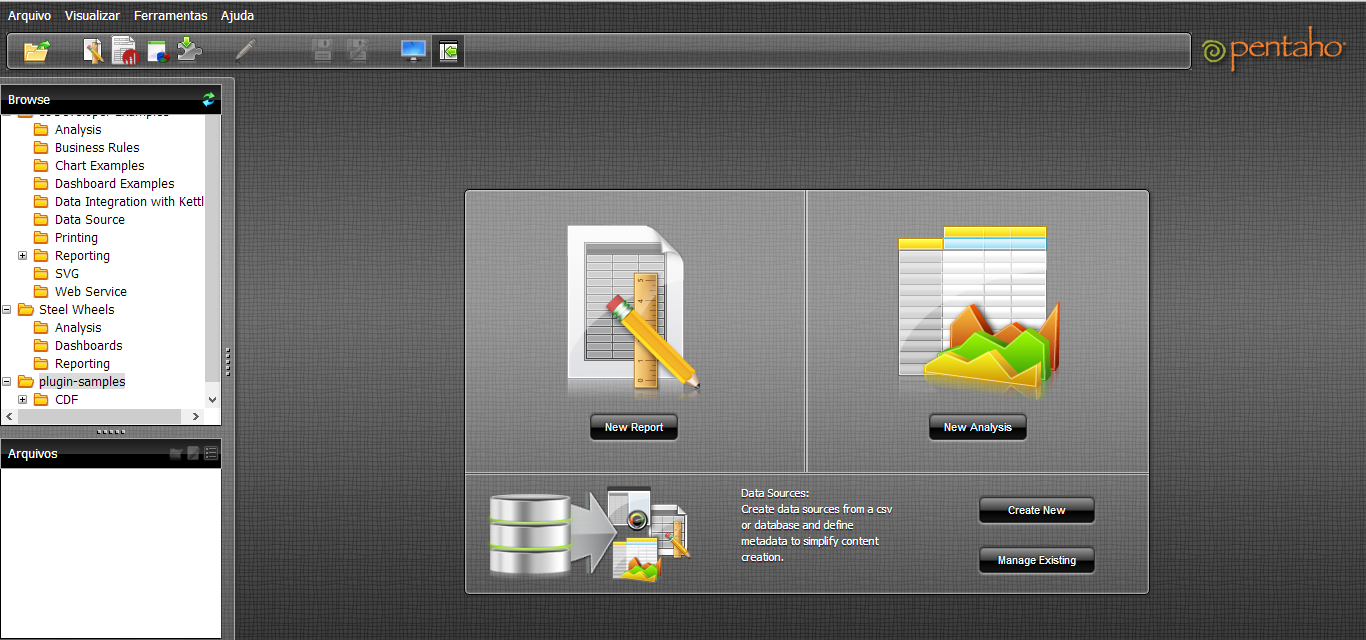
\includegraphics[keepaspectratio=true, scale=0.45]{figuras/pentahoBI.eps}
\caption{Interface Gráfica do Pentaho BI Platform}
\label{BIplatform}
\end{center}
\end{figure}
\FloatBarrier
 

A ferramenta Pentaho BI Platform possui arquitetura extensível por plugins diversos que realizam diversas operações, tais como, criação de relatórios, visualização dos dados em tabelas e gráficos e entre outros. Entre os plugins disponíveis, está o Saiku Analytics que oferece serviços de apoio a operações OLAP e à visualização de dados. As características gerais do Saiku Analytics, bem como a avaliação quanto aos critérios gerais de seleção de ferramentas, são apresentados na Tabela \ref{saiku}. 

\begin{table}[!ht]
\begin{tabular}{|p{4.5cm}|p{5.0cm}|p{1cm}|p{1cm}|p{1cm}|p{1cm}|}
\hline
Característica                                          

&


\begin{center}

\includegraphics[keepaspectratio=false,scale=0.4]{figuras/saiku_olap_logo.eps} 
\end{center}                                              

& CG01 

& CG02       

& CG03       


& CG04       


\\ \hline

Licença                                                 & GPL 2.0                              & \checkmark &            &            &            \\ \hline
Componentes de Visualização                           & Tabelas e Gráficos &            &            &            &            \\ \hline
Gráficos com Suporte & Gráfico de Pizza, Gráfico de Linhas, Gráfico de Área, Gráfico de Setor e entre outros &            &            &            &

 \\ \hline
Ultima Versão Estável (10/05/2014)                      & 2.8                                             &            &            &            & \checkmark \\ \hline
Quantidade de Commits no Repositório Oficial em 14/11/2013            & 790                                         &            &            & \checkmark &            \\ \hline
Idioma da Documentação                                  & Inglês                                          &            & \checkmark &            &            \\ \hline            
Quantidade de Casos Abertos no \textit{Issue Tracker} & 227                                           &&            & \checkmark &            \\ \hline

\end{tabular}
\caption{Características do Saiku Analytics e avaliação quanto aos critérios gerais de seleção de ferramentas}
\label{saiku}
\end{table}
\FloatBarrier


O Saiku Analytics possui em sua arquitetura outro componente da arquitetura do Pentaho BI Suite, que é o Mondrian OLAP Server. Este permite ao Saiku, que sejam realizadas consultas \textit{ad hoc} com as dimensões do cubo, de um esquema dimensional, realizando \textit{drag and drop} das colunas das dimensões.

Por meio do Saiku, permite-se a realização de consultas. Estas ocorrem por meio da escrita de \textit{queries} em linguagem MDX \textit{(MulitDimensional eXpressions)}. Esta foi proposta por \citeonline{spofford2006mdx} como uma forma de escrever consultas mais otimizadas para bases seguem o modelo dimensional, tal como mostra o exemplo do trecho de Código-Fonte \ref{MDX}.




\begin{center}
\begin{minipage}{0.5\textwidth}

\begin{lstlisting}[caption=Exemplo de \textit{Query} em linguagem MDX, label=MDX]
 SELECT
   { [Measures].[Loja] } ON COLUMNS,
   { [Tempo].[2002], [Tempo].[2003] } ON ROWS
FROM Vendas
WHERE ( [Loja].[Loja Sul]) 

\end{lstlisting}
\end{minipage}
\end{center}
\FloatBarrier


 
